
% Default to the notebook output style

    


% Inherit from the specified cell style.




    
\documentclass{article}

    
    
    \usepackage{graphicx} % Used to insert images
    \usepackage{adjustbox} % Used to constrain images to a maximum size 
    \usepackage{color} % Allow colors to be defined
    \usepackage{enumerate} % Needed for markdown enumerations to work
    \usepackage{geometry} % Used to adjust the document margins
    \usepackage{amsmath} % Equations
    \usepackage{amssymb} % Equations
    \usepackage{eurosym} % defines \euro
    \usepackage[mathletters]{ucs} % Extended unicode (utf-8) support
    \usepackage[utf8x]{inputenc} % Allow utf-8 characters in the tex document
    \usepackage{fancyvrb} % verbatim replacement that allows latex
    \usepackage{grffile} % extends the file name processing of package graphics 
                         % to support a larger range 
    % The hyperref package gives us a pdf with properly built
    % internal navigation ('pdf bookmarks' for the table of contents,
    % internal cross-reference links, web links for URLs, etc.)
    \usepackage{hyperref}
    \usepackage{longtable} % longtable support required by pandoc >1.10
    \usepackage{booktabs}  % table support for pandoc > 1.12.2
    \usepackage{indentfirst}
    \usepackage{amsmath}
    \usepackage{floatrow}
    
    
    \definecolor{orange}{cmyk}{0,0.4,0.8,0.2}
    \definecolor{darkorange}{rgb}{.71,0.21,0.01}
    \definecolor{darkgreen}{rgb}{.12,.54,.11}
    \definecolor{myteal}{rgb}{.26, .44, .56}
    \definecolor{gray}{gray}{0.45}
    \definecolor{lightgray}{gray}{.95}
    \definecolor{mediumgray}{gray}{.8}
    \definecolor{inputbackground}{rgb}{.95, .95, .85}
    \definecolor{outputbackground}{rgb}{.95, .95, .95}
    \definecolor{traceback}{rgb}{1, .95, .95}
    % ansi colors
    \definecolor{red}{rgb}{.6,0,0}
    \definecolor{green}{rgb}{0,.65,0}
    \definecolor{brown}{rgb}{0.6,0.6,0}
    \definecolor{blue}{rgb}{0,.145,.698}
    \definecolor{purple}{rgb}{.698,.145,.698}
    \definecolor{cyan}{rgb}{0,.698,.698}
    \definecolor{lightgray}{gray}{0.5}
    
    % bright ansi colors
    \definecolor{darkgray}{gray}{0.25}
    \definecolor{lightred}{rgb}{1.0,0.39,0.28}
    \definecolor{lightgreen}{rgb}{0.48,0.99,0.0}
    \definecolor{lightblue}{rgb}{0.53,0.81,0.92}
    \definecolor{lightpurple}{rgb}{0.87,0.63,0.87}
    \definecolor{lightcyan}{rgb}{0.5,1.0,0.83}
    
    % commands and environments needed by pandoc snippets
    % extracted from the output of `pandoc -s`
    \providecommand{\tightlist}{%
      \setlength{\itemsep}{0pt}\setlength{\parskip}{0pt}}
    \DefineVerbatimEnvironment{Highlighting}{Verbatim}{commandchars=\\\{\}}
    % Add ',fontsize=\small' for more characters per line
    \newenvironment{Shaded}{}{}
    \newcommand{\KeywordTok}[1]{\textcolor[rgb]{0.00,0.44,0.13}{\textbf{{#1}}}}
    \newcommand{\DataTypeTok}[1]{\textcolor[rgb]{0.56,0.13,0.00}{{#1}}}
    \newcommand{\DecValTok}[1]{\textcolor[rgb]{0.25,0.63,0.44}{{#1}}}
    \newcommand{\BaseNTok}[1]{\textcolor[rgb]{0.25,0.63,0.44}{{#1}}}
    \newcommand{\FloatTok}[1]{\textcolor[rgb]{0.25,0.63,0.44}{{#1}}}
    \newcommand{\CharTok}[1]{\textcolor[rgb]{0.25,0.44,0.63}{{#1}}}
    \newcommand{\StringTok}[1]{\textcolor[rgb]{0.25,0.44,0.63}{{#1}}}
    \newcommand{\CommentTok}[1]{\textcolor[rgb]{0.38,0.63,0.69}{\textit{{#1}}}}
    \newcommand{\OtherTok}[1]{\textcolor[rgb]{0.00,0.44,0.13}{{#1}}}
    \newcommand{\AlertTok}[1]{\textcolor[rgb]{1.00,0.00,0.00}{\textbf{{#1}}}}
    \newcommand{\FunctionTok}[1]{\textcolor[rgb]{0.02,0.16,0.49}{{#1}}}
    \newcommand{\RegionMarkerTok}[1]{{#1}}
    \newcommand{\ErrorTok}[1]{\textcolor[rgb]{1.00,0.00,0.00}{\textbf{{#1}}}}
    \newcommand{\NormalTok}[1]{{#1}}
    
    % Define a nice break command that doesn't care if a line doesn't already
    % exist.
    \def\br{\hspace*{\fill} \\* }
    % Math Jax compatability definitions
    \def\gt{>}
    \def\lt{<}
    % Document parameters
    \title{Homework 10}
    \author{Roly Vicar\'ia \\ STAT501 Fall 2015}
    
    

    % Pygments definitions
    
\makeatletter
\def\PY@reset{\let\PY@it=\relax \let\PY@bf=\relax%
    \let\PY@ul=\relax \let\PY@tc=\relax%
    \let\PY@bc=\relax \let\PY@ff=\relax}
\def\PY@tok#1{\csname PY@tok@#1\endcsname}
\def\PY@toks#1+{\ifx\relax#1\empty\else%
    \PY@tok{#1}\expandafter\PY@toks\fi}
\def\PY@do#1{\PY@bc{\PY@tc{\PY@ul{%
    \PY@it{\PY@bf{\PY@ff{#1}}}}}}}
\def\PY#1#2{\PY@reset\PY@toks#1+\relax+\PY@do{#2}}

\expandafter\def\csname PY@tok@gd\endcsname{\def\PY@tc##1{\textcolor[rgb]{0.63,0.00,0.00}{##1}}}
\expandafter\def\csname PY@tok@gu\endcsname{\let\PY@bf=\textbf\def\PY@tc##1{\textcolor[rgb]{0.50,0.00,0.50}{##1}}}
\expandafter\def\csname PY@tok@gt\endcsname{\def\PY@tc##1{\textcolor[rgb]{0.00,0.27,0.87}{##1}}}
\expandafter\def\csname PY@tok@gs\endcsname{\let\PY@bf=\textbf}
\expandafter\def\csname PY@tok@gr\endcsname{\def\PY@tc##1{\textcolor[rgb]{1.00,0.00,0.00}{##1}}}
\expandafter\def\csname PY@tok@cm\endcsname{\let\PY@it=\textit\def\PY@tc##1{\textcolor[rgb]{0.25,0.50,0.50}{##1}}}
\expandafter\def\csname PY@tok@vg\endcsname{\def\PY@tc##1{\textcolor[rgb]{0.10,0.09,0.49}{##1}}}
\expandafter\def\csname PY@tok@m\endcsname{\def\PY@tc##1{\textcolor[rgb]{0.40,0.40,0.40}{##1}}}
\expandafter\def\csname PY@tok@mh\endcsname{\def\PY@tc##1{\textcolor[rgb]{0.40,0.40,0.40}{##1}}}
\expandafter\def\csname PY@tok@go\endcsname{\def\PY@tc##1{\textcolor[rgb]{0.53,0.53,0.53}{##1}}}
\expandafter\def\csname PY@tok@ge\endcsname{\let\PY@it=\textit}
\expandafter\def\csname PY@tok@vc\endcsname{\def\PY@tc##1{\textcolor[rgb]{0.10,0.09,0.49}{##1}}}
\expandafter\def\csname PY@tok@il\endcsname{\def\PY@tc##1{\textcolor[rgb]{0.40,0.40,0.40}{##1}}}
\expandafter\def\csname PY@tok@cs\endcsname{\let\PY@it=\textit\def\PY@tc##1{\textcolor[rgb]{0.25,0.50,0.50}{##1}}}
\expandafter\def\csname PY@tok@cp\endcsname{\def\PY@tc##1{\textcolor[rgb]{0.74,0.48,0.00}{##1}}}
\expandafter\def\csname PY@tok@gi\endcsname{\def\PY@tc##1{\textcolor[rgb]{0.00,0.63,0.00}{##1}}}
\expandafter\def\csname PY@tok@gh\endcsname{\let\PY@bf=\textbf\def\PY@tc##1{\textcolor[rgb]{0.00,0.00,0.50}{##1}}}
\expandafter\def\csname PY@tok@ni\endcsname{\let\PY@bf=\textbf\def\PY@tc##1{\textcolor[rgb]{0.60,0.60,0.60}{##1}}}
\expandafter\def\csname PY@tok@nl\endcsname{\def\PY@tc##1{\textcolor[rgb]{0.63,0.63,0.00}{##1}}}
\expandafter\def\csname PY@tok@nn\endcsname{\let\PY@bf=\textbf\def\PY@tc##1{\textcolor[rgb]{0.00,0.00,1.00}{##1}}}
\expandafter\def\csname PY@tok@no\endcsname{\def\PY@tc##1{\textcolor[rgb]{0.53,0.00,0.00}{##1}}}
\expandafter\def\csname PY@tok@na\endcsname{\def\PY@tc##1{\textcolor[rgb]{0.49,0.56,0.16}{##1}}}
\expandafter\def\csname PY@tok@nb\endcsname{\def\PY@tc##1{\textcolor[rgb]{0.00,0.50,0.00}{##1}}}
\expandafter\def\csname PY@tok@nc\endcsname{\let\PY@bf=\textbf\def\PY@tc##1{\textcolor[rgb]{0.00,0.00,1.00}{##1}}}
\expandafter\def\csname PY@tok@nd\endcsname{\def\PY@tc##1{\textcolor[rgb]{0.67,0.13,1.00}{##1}}}
\expandafter\def\csname PY@tok@ne\endcsname{\let\PY@bf=\textbf\def\PY@tc##1{\textcolor[rgb]{0.82,0.25,0.23}{##1}}}
\expandafter\def\csname PY@tok@nf\endcsname{\def\PY@tc##1{\textcolor[rgb]{0.00,0.00,1.00}{##1}}}
\expandafter\def\csname PY@tok@si\endcsname{\let\PY@bf=\textbf\def\PY@tc##1{\textcolor[rgb]{0.73,0.40,0.53}{##1}}}
\expandafter\def\csname PY@tok@s2\endcsname{\def\PY@tc##1{\textcolor[rgb]{0.73,0.13,0.13}{##1}}}
\expandafter\def\csname PY@tok@vi\endcsname{\def\PY@tc##1{\textcolor[rgb]{0.10,0.09,0.49}{##1}}}
\expandafter\def\csname PY@tok@nt\endcsname{\let\PY@bf=\textbf\def\PY@tc##1{\textcolor[rgb]{0.00,0.50,0.00}{##1}}}
\expandafter\def\csname PY@tok@nv\endcsname{\def\PY@tc##1{\textcolor[rgb]{0.10,0.09,0.49}{##1}}}
\expandafter\def\csname PY@tok@s1\endcsname{\def\PY@tc##1{\textcolor[rgb]{0.73,0.13,0.13}{##1}}}
\expandafter\def\csname PY@tok@kd\endcsname{\let\PY@bf=\textbf\def\PY@tc##1{\textcolor[rgb]{0.00,0.50,0.00}{##1}}}
\expandafter\def\csname PY@tok@sh\endcsname{\def\PY@tc##1{\textcolor[rgb]{0.73,0.13,0.13}{##1}}}
\expandafter\def\csname PY@tok@sc\endcsname{\def\PY@tc##1{\textcolor[rgb]{0.73,0.13,0.13}{##1}}}
\expandafter\def\csname PY@tok@sx\endcsname{\def\PY@tc##1{\textcolor[rgb]{0.00,0.50,0.00}{##1}}}
\expandafter\def\csname PY@tok@bp\endcsname{\def\PY@tc##1{\textcolor[rgb]{0.00,0.50,0.00}{##1}}}
\expandafter\def\csname PY@tok@c1\endcsname{\let\PY@it=\textit\def\PY@tc##1{\textcolor[rgb]{0.25,0.50,0.50}{##1}}}
\expandafter\def\csname PY@tok@kc\endcsname{\let\PY@bf=\textbf\def\PY@tc##1{\textcolor[rgb]{0.00,0.50,0.00}{##1}}}
\expandafter\def\csname PY@tok@c\endcsname{\let\PY@it=\textit\def\PY@tc##1{\textcolor[rgb]{0.25,0.50,0.50}{##1}}}
\expandafter\def\csname PY@tok@mf\endcsname{\def\PY@tc##1{\textcolor[rgb]{0.40,0.40,0.40}{##1}}}
\expandafter\def\csname PY@tok@err\endcsname{\def\PY@bc##1{\setlength{\fboxsep}{0pt}\fcolorbox[rgb]{1.00,0.00,0.00}{1,1,1}{\strut ##1}}}
\expandafter\def\csname PY@tok@mb\endcsname{\def\PY@tc##1{\textcolor[rgb]{0.40,0.40,0.40}{##1}}}
\expandafter\def\csname PY@tok@ss\endcsname{\def\PY@tc##1{\textcolor[rgb]{0.10,0.09,0.49}{##1}}}
\expandafter\def\csname PY@tok@sr\endcsname{\def\PY@tc##1{\textcolor[rgb]{0.73,0.40,0.53}{##1}}}
\expandafter\def\csname PY@tok@mo\endcsname{\def\PY@tc##1{\textcolor[rgb]{0.40,0.40,0.40}{##1}}}
\expandafter\def\csname PY@tok@kn\endcsname{\let\PY@bf=\textbf\def\PY@tc##1{\textcolor[rgb]{0.00,0.50,0.00}{##1}}}
\expandafter\def\csname PY@tok@mi\endcsname{\def\PY@tc##1{\textcolor[rgb]{0.40,0.40,0.40}{##1}}}
\expandafter\def\csname PY@tok@gp\endcsname{\let\PY@bf=\textbf\def\PY@tc##1{\textcolor[rgb]{0.00,0.00,0.50}{##1}}}
\expandafter\def\csname PY@tok@o\endcsname{\def\PY@tc##1{\textcolor[rgb]{0.40,0.40,0.40}{##1}}}
\expandafter\def\csname PY@tok@kr\endcsname{\let\PY@bf=\textbf\def\PY@tc##1{\textcolor[rgb]{0.00,0.50,0.00}{##1}}}
\expandafter\def\csname PY@tok@s\endcsname{\def\PY@tc##1{\textcolor[rgb]{0.73,0.13,0.13}{##1}}}
\expandafter\def\csname PY@tok@kp\endcsname{\def\PY@tc##1{\textcolor[rgb]{0.00,0.50,0.00}{##1}}}
\expandafter\def\csname PY@tok@w\endcsname{\def\PY@tc##1{\textcolor[rgb]{0.73,0.73,0.73}{##1}}}
\expandafter\def\csname PY@tok@kt\endcsname{\def\PY@tc##1{\textcolor[rgb]{0.69,0.00,0.25}{##1}}}
\expandafter\def\csname PY@tok@ow\endcsname{\let\PY@bf=\textbf\def\PY@tc##1{\textcolor[rgb]{0.67,0.13,1.00}{##1}}}
\expandafter\def\csname PY@tok@sb\endcsname{\def\PY@tc##1{\textcolor[rgb]{0.73,0.13,0.13}{##1}}}
\expandafter\def\csname PY@tok@k\endcsname{\let\PY@bf=\textbf\def\PY@tc##1{\textcolor[rgb]{0.00,0.50,0.00}{##1}}}
\expandafter\def\csname PY@tok@se\endcsname{\let\PY@bf=\textbf\def\PY@tc##1{\textcolor[rgb]{0.73,0.40,0.13}{##1}}}
\expandafter\def\csname PY@tok@sd\endcsname{\let\PY@it=\textit\def\PY@tc##1{\textcolor[rgb]{0.73,0.13,0.13}{##1}}}

\def\PYZbs{\char`\\}
\def\PYZus{\char`\_}
\def\PYZob{\char`\{}
\def\PYZcb{\char`\}}
\def\PYZca{\char`\^}
\def\PYZam{\char`\&}
\def\PYZlt{\char`\<}
\def\PYZgt{\char`\>}
\def\PYZsh{\char`\#}
\def\PYZpc{\char`\%}
\def\PYZdl{\char`\$}
\def\PYZhy{\char`\-}
\def\PYZsq{\char`\'}
\def\PYZdq{\char`\"}
\def\PYZti{\char`\~}
% for compatibility with earlier versions
\def\PYZat{@}
\def\PYZlb{[}
\def\PYZrb{]}
\makeatother


    % Exact colors from NB
    \definecolor{incolor}{rgb}{0.0, 0.0, 0.5}
    \definecolor{outcolor}{rgb}{0.545, 0.0, 0.0}



    
    % Prevent overflowing lines due to hard-to-break entities
    \sloppy 
    % Setup hyperref package
    \hypersetup{
      breaklinks=true,  % so long urls are correctly broken across lines
      colorlinks=true,
      urlcolor=blue,
      linkcolor=darkorange,
      citecolor=darkgreen,
      }
    % Slightly bigger margins than the latex defaults
    
    \geometry{verbose,tmargin=1in,bmargin=1in,lmargin=1in,rmargin=1in}
    
    

    \begin{document}
    
    
    \maketitle
    
    

    
    \subsubsection{Question 1}\label{question-1}

\begin{enumerate}
\def\labelenumi{\alph{enumi})}
\item
  \(Weight = -158.8 + 16.95 Neck\); MSE = 1610
\item
  Bear number 13 has the highest leverage: 0.286265
\item
  \(3(p/n) = 3(2/19) = 0.316\); The leverage from the part (b) is less
  than the threshold.
\item
  \(Weight = -158.8 + 16.95 (10.5) = 19.175\); Minitab FITS1 value:
  19.171
\item
  \(Residual = 140 - 19.175 = 120.825\); Minitab RESI1 value: 120.829
\item
  Leverage of bear \#6 = 0.239605
\item
  \(r_6 = \frac{e_6}{\sqrt{MSE (1 - h_{66})}} = \frac{120.825}{\sqrt{1610 (1 - 0.239605)}} = 3.453\);
  Minitab SRES1 value: 3.45320
\item
  \(Weight = -234.6 + 20.54 Neck\); MSE = 511
\item
  \(t_6 = \frac{e_6}{\sqrt{MSE (1 - h_{66})}} = \frac{120.825}{\sqrt{511 (1 - 0.239605)}} = 6.130\);
  Minitab TRES1 value: 6.13120
\item
  \(Weight = -234.6 + 20.54 (10.5) = -18.93\)
\item
  \(DFITS_6 = \frac{\hat{y}_6 - \hat{y}_{(6)}}{\sqrt{MSE_{(6)}h_{66}}} = \frac{19.175 - (-18.93)}{\sqrt{511 (0.239605)}} = 3.444\);
  Minitab DFIT1 value: 3.44171
\item
  \(2\sqrt{\frac{p + 1}{n - p - 1}} = 2\sqrt{\frac{2 + 1}{19 - 2 - 1}} = 0.866\);
  Yes, the absolute value of the value from part (k) is greater than the
  threshold given in the online notes.
\item
  \(D_6 = \frac{(y_6 - \hat{y}_6)^2}{p \times MSE} \left[\frac{h_{66}}{(1 - h_{66})^2}\right] = \frac{120.825^2}{2 \times 1610} \left[\frac{0.239605}{(1 - 0.239605)^2}\right] = 1.879\);
  Minitab COOK1 value: 1.87875
\item
  Yes, the Cook's distance is greater than 1 which indicates a high
  likelihood of being an influential point. It is also much greater than
  the Cook's distance of any other point which further supports the
  likelihood of it being influential.
  \newpage
\item
  The Cook's distance and the DFITS values for bear \#6 both indicate
  that it's an outlier and influential point. The model fitted excluding
  bear 6 showed a much better MSE. It looks like deleting bear 6 was the
  correct action to take. It narrowed down the scope of the model to
  bears with weight greater than 12.
  
  \begin{figure}[!h]
  \begin{floatrow}
   \ffigbox{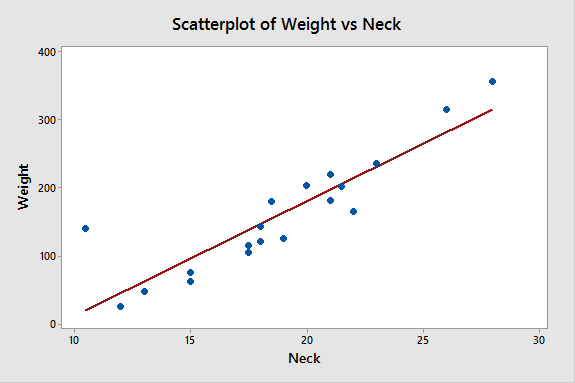
\includegraphics[scale=0.5]{./images/scatterplot-with-regression_weight-vs-neck.png}}{}
   \ffigbox{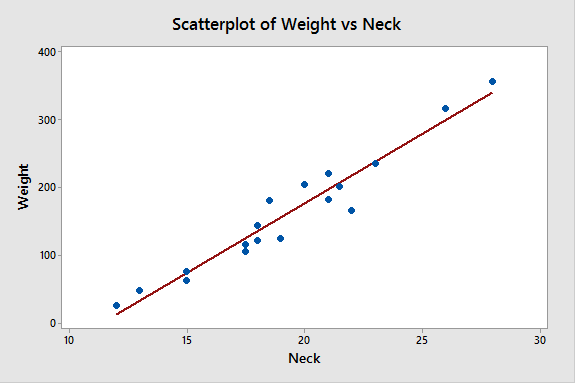
\includegraphics[scale=0.5]{./images/scatterplot-with-regression_weight-vs-neck_excluding-obs6.png}}{}
  \end{floatrow}
\end{figure}
\end{enumerate}

    \subsubsection{Question 2}\label{question-2}

\begin{enumerate}
\def\labelenumi{\alph{enumi})}
\item
  \(Gpa = -7.22 + 0.1263 Verb + 0.1170 Math - 0.001130 Verb^2 - 0.001063 Math^2 + 0.000878 Verb*Math\)
\item
  Student 28 has the highest absolute externally studentized residual:
  -3.03046
\item
  Yes, the absolute value of the result from part (b) is greater than 3.
  Therefore we would call this observation an outlier.
\item
  Student 4 has the highest leverage: 0.563070
\item
  \(3(p/n) = 3(6/40) = 0.45\); Yes, the leverage from part (d) is
  greater than the threshold.
\item
  The range of observed Verbal scores is {[}39, 100{]} and the range of
  observed Math scores is {[}49, 99{]}. Student 4 has a Verbal score of
  100 and a Math score of 49. They are the upper extreme of Verbal
  scores and the lower extreme of Math scores.
\item
  Student 9 has the highest Cook's distance: 0.308919
\item
  No, the Cook's distance from part (g) is not higher than the threshold
  given in the notes.
  
\newpage
\item
  With all students:

\begin{verbatim}
Model Summary

       S    R-sq  R-sq(adj)  R-sq(pred)

0.203390  93.05%     92.03%      89.94%

Coefficients

Term            Coef   SE Coef  T-Value  P-Value     VIF
Constant       -7.22      1.47    -4.91    0.000
Verb          0.1263    0.0231     5.47    0.000  130.31 
Math          0.1170    0.0291     4.03    0.000  137.59 
Verb*Verb  -0.001130  0.000127    -8.87    0.000   82.80 
Math*Math  -0.001063  0.000173    -6.14    0.000  107.87 
Verb*Math   0.000878  0.000156     5.61    0.000   47.03

Regression Equation

Gpa = -7.22 + 0.1263 Verb + 0.1170 Math - 0.001130 Verb*Verb - 0.001063 Math*Math 
         + 0.000878 Verb*Math
  \end{verbatim}
  
Excluding student 28:

\begin{verbatim}
Model Summary

       S    R-sq  R-sq(adj)  R-sq(pred)
0.182598  94.52%     93.69%      91.31%

Coefficients

Term            Coef   SE Coef  T-Value  P-Value     VIF
Constant       -7.28      1.32    -5.50    0.000
Verb          0.1156    0.0210     5.50    0.000  124.95
Math          0.1275    0.0263     4.85    0.000  138.96
Verb*Verb  -0.001033  0.000119    -8.69    0.000   81.81
Math*Math  -0.001123  0.000157    -7.16    0.000  108.62
Verb*Math   0.000854  0.000141     6.07    0.000   46.23

Regression Equation

Gpa = -7.28 + 0.1156 Verb + 0.1275 Math - 0.001033 Verb*Verb - 0.001123 Math*Math 
         + 0.000854 Verb*Math
\end{verbatim}

Removing observation for student 28 does not affect the \(R^2\) very
much. It's still a strong relationship. The standard error of all
coefficients decreased marginally. The most notable difference is that
the MSE decreased from 0.04137 to 0.03334. Therefore
confidence/prediction intervals will be narrower in the model excluding
28.

\newpage
Excluding student 4:

\begin{verbatim}
Model Summary

       S    R-sq  R-sq(adj)  R-sq(pred)
0.206400  92.20%     91.01%      87.00%

Coefficients

Term            Coef   SE Coef  T-Value  P-Value     VIF
Constant       -7.20      1.50    -4.79    0.000
Verb          0.1265    0.0235     5.38    0.000  120.94
Math          0.1162    0.0303     3.83    0.001  131.55
Verb*Verb  -0.001125  0.000135    -8.32    0.000   81.40
Math*Math  -0.001052  0.000196    -5.36    0.000  124.84
Verb*Math   0.000866  0.000186     4.67    0.000   64.09

Regression Equation

Gpa = -7.20 + 0.1265 Verb + 0.1162 Math - 0.001125 Verb*Verb - 0.001052 Math*Math
         + 0.000866 Verb*Math
\end{verbatim}

Removing observation for student 4 has a small decrease in \(R^2\), but
still a strong relationship. All the coefficients show marginal
increase, but nothing to affect p-value of any of them. The MSE actually
increased a little bit, from 0.04137 to 0.04260. That means that
confidence/prediction intervals based on this model will be slightly
wider than the original model.
\\

Excluding student 9:

\begin{verbatim}
Model Summary

       S    R-sq  R-sq(adj)  R-sq(pred)
0.186187  93.76%     92.82%      91.13%

Coefficients

Term            Coef   SE Coef  T-Value  P-Value     VIF
Constant       -5.81      1.44    -4.03    0.000
Verb          0.1163    0.0214     5.43    0.000  130.12
Math          0.0912    0.0282     3.23    0.003  145.29
Verb*Verb  -0.001127  0.000117    -9.66    0.000   80.44
Math*Math  -0.000957  0.000163    -5.86    0.000  108.39
Verb*Math   0.000994  0.000149     6.66    0.000   47.46

Regression Equation

Gpa = -5.81 + 0.1163 Verb + 0.0912 Math - 0.001127 Verb*Verb - 0.000957 Math*Math 
         + 0.000994 Verb*Math
\end{verbatim}

Removing observation for student 9 has very little effect on the \(R^2\)
value, still a strong relationship. It had a noticeable impact on the
estimated coefficient \(b_0\), from -7.22 in the original model to -5.81
in this model. The value for \(b_1\) also saw a relatively significant
decrease. The MSE of this model is lower than the original, 0.03467
compared to 0.04137 of the original. So this model would show narrower
confidence/prediction intervals.

Overall, the impacts of removing these observations seem small. They
show some improvement, but none that look very significant to me. The
difference in MSE by removing observation 9 was the most significant
difference in my opinion.
\end{enumerate}

    \subsubsection{Question 3}\label{question-3}

\begin{enumerate}
\def\labelenumi{\alph{enumi})}
\tightlist
\item
  The scatterplot of lnPSA vs lnCanVol shows a positive relationship
  between lnPSA and lnCanVol. All the data points seem to follow the
  same general trend. The scatterplot of lnPSA vs Weight also shows a
  positive relationship. This plot, however, shows a handful of points
  that appear to stray from the general trend. At least one definite
  outlier.
  
  \begin{figure}[!h]
  \begin{floatrow}
   \ffigbox{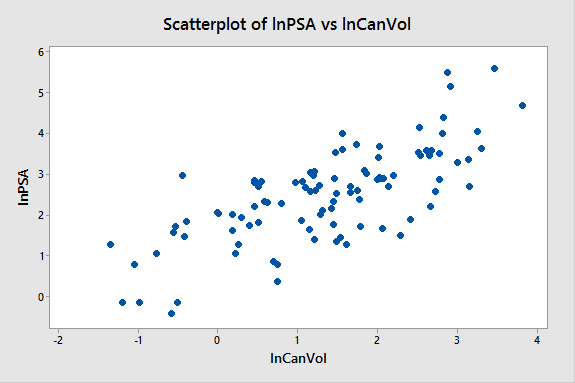
\includegraphics[scale=0.5]{./images/scatterplot_lnPSA-vs-lnCanVol.png}}{}
   \ffigbox{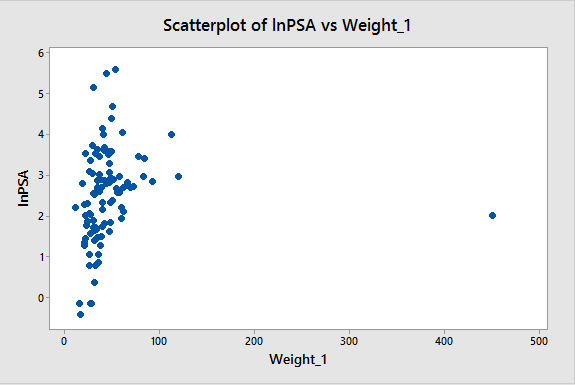
\includegraphics[scale=0.5]{./images/scatterplot_lnPSA-vs-Weight.png}}{}
  \end{floatrow}
\end{figure}
\end{enumerate}

\begin{enumerate}
\def\labelenumi{\alph{enumi})}
\setcounter{enumi}{1}
\item
\end{enumerate}

\begin{longtable}[c]{@{}llll@{}}
\toprule
Predictor & Coefficient value & Standard error &
\emph{p}-value\tabularnewline
\midrule
\endhead
lnCanVol & 0.7183 & 0.0675 & 0.000\tabularnewline
Weight & 0.00307 & 0.00174 & 0.081\tabularnewline
\bottomrule
\end{longtable}

\begin{enumerate}
\def\labelenumi{\alph{enumi})}
\setcounter{enumi}{2}
\tightlist
\item
  Plot of \(X_1\) vs \(X_2\):

\begin{figure}[h!]
 \centering
 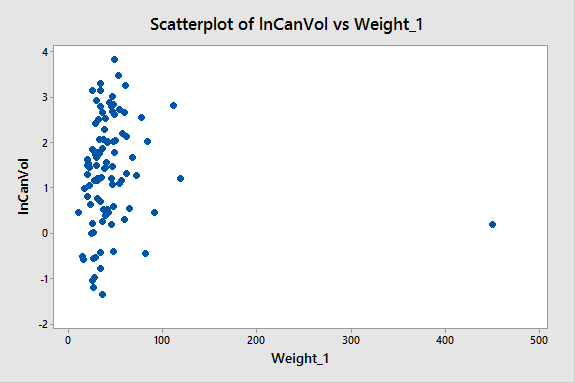
\includegraphics[scale=.5]{./images/scatterplot_lnCanVol-vs-Weight.png}
 % scatterplot_lnCanVol-vs-Weight.png: 575x383 pixel, 96dpi, 15.21x10.13 cm, bb=0 0 431 287
\end{figure}

The majority of the observations flagged by Minitab are marked with `R'
indicating an internally studentized residual greater than 2. These are
``unusual'' y values that could potentially be outliers. The observation
marked with an `R' and an `X' indicates an ``usual'' y value AND an
``unusual'' x value. Indeed, we can see in all the plots that this
observation has a weight = 450 which is much larger than all other
weight values. Of the flagged observations, the only clear outlier is
observation 32. The others are potential outliers that require further
investigation.
\end{enumerate}

\begin{enumerate}
\def\labelenumi{\alph{enumi})}
\setcounter{enumi}{3}
\tightlist
\item
  DFITS threshold:
  \(2 \sqrt{\frac{p + 1}{n - p -1}} = 2 \sqrt{\frac{3 + 1}{97 - 3 - 1}} = 0.4148\)

Observations with Cook's distance greater than 1:

\begin{verbatim}
        Observation 32
\end{verbatim}

Observations with DFITS greater than 0.4148:

\begin{verbatim}
        Observation 32
        Observation 69
        Observation 96
        Observation 97
\end{verbatim}

Of these observations, the only one I would consider deleting is
observation 32. It is clearly an outlier by any measure. By deleting
this observation, we would be narrowing down the scope of the model. The
other observations with high DFITS values are over the threshold, but do
not stick out like sore thumbs. There are other values just below that
threshold as well, so I do not think they warrant any action.
\end{enumerate}

\begin{enumerate}
\def\labelenumi{\alph{enumi})}
\setcounter{enumi}{4}
\item
\end{enumerate}

\begin{longtable}[c]{@{}llll@{}}
\toprule
Predictor & Coefficient value & Standard error &
\emph{p}-value\tabularnewline
\midrule
\endhead
lnCanVol & 0.6711 & 0.0670 & 0.000\tabularnewline
Weight & 0.01393 & 0.00412 & 0.001\tabularnewline
\bottomrule
\end{longtable}

The model computed after removing observation 32 had a small effect on
the value of the lnCanVol coefficient. The standard error and
\emph{p}-value remained the same, however. The change to the coefficient
on Weight was more significant, from 0.00307 to 0.01393. The
\emph{p}-value for the Weight coefficient also changed significantly.
Under the original model, the \emph{p}-value would have indicated that
\(\beta_2 = 0\). The model excluding observation 32 has changed the
outcome of that hypothesis test.

\begin{enumerate}
\def\labelenumi{\alph{enumi})}
\setcounter{enumi}{5}
\item
  The plot of residuals vs fits for the model in part (e) does not
  indicate any difficulties. It has a good horizontal band shape around
  the residual = 0 line. The spread of points around the line indicate
  constant and even distribution of errors.
  
  \begin{figure}[h!]
 \centering
 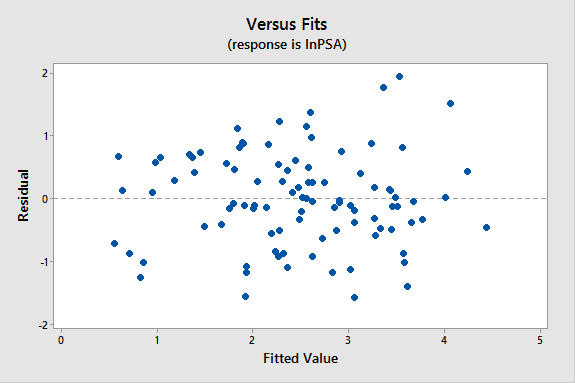
\includegraphics[scale=.5]{./images/scatterplot_residual-vs-fits_model-excluding-obs32.png}
 % scatterplot_residual-vs-fits_model-excluding-obs32.png: 575x383 pixel, 96dpi, 15.21x10.13 cm, bb=0 0 431 287
\end{figure}

\newpage  
\item
  DFITS threshold:
  \(2 \sqrt{\frac{p + 1}{n - p -1}} = 2 \sqrt{\frac{3 + 1}{96 - 3 - 1}} = 0.417\)

Observations with Cook's distance greater than 1:

\begin{verbatim}
        None
\end{verbatim}

Observations with DFITS greater than 0.417:

\begin{verbatim}
        Observation 69
        Observation 95
        Observation 96
        Observation 97
\end{verbatim}

Of the observations with DFITS values over the threshold, I tried
fitting a model removing observation 69, and it didn't seem to have a
positive effect on the model. The t-value of the Weight coefficient
actually went down a little. As I said in part (d), I don't think that
any of the flagged observations warrant any action. The residuals vs
fits plot doesn't indicate any difficulties with the model.
\end{enumerate}

    % Add a bibliography block to the postdoc
    
    
    
    \end{document}
